\chapter{SNN模型结构}
\par
有两种方法可以改善通过转换获得的SNN的性能:一是在转换之前训练更好的ANN,二是通过消除SNN的近似误差来改善转换。后者在前一章节中给出了理论方法。而训练更好的ANN,目前用于目标检测且推理速度较快的模型主要是单阶段检测(one-stage detction):主要代表有ssd和yolo两类,因此我们选用这两类作为转换前的基础ANN
\section{spiking-ssd}
\par
首先介绍在ssd上进行的脉冲神经网络转化,即借用ssd的网络模型进行脉冲转化操作,
我们称之为"spiking-ssd"。ssd的具体结构我们已经在第三章中讲过,以下主要是阐述我们进行转化的网络模型。
\par
转换的核心是用脉冲神经元的脉冲发放频率代替人工神经网络中的激活值。
主要步骤如下:首先使用反向传播算法训练ANN(即ssd)达到较好性能,
然后将ANN中的BatchNorm层与前一层的卷积层进行融合,
根据每层的等效最大值对权重和偏置进行归一化,
并映射到具有相同拓扑结构的脉冲神经网络中,确保转换过程的信息损失最小。
实验方法流程如下图:
\begin{figure}[H]
	\centering
	\setlength{\abovecaptionskip}{0cm}  
	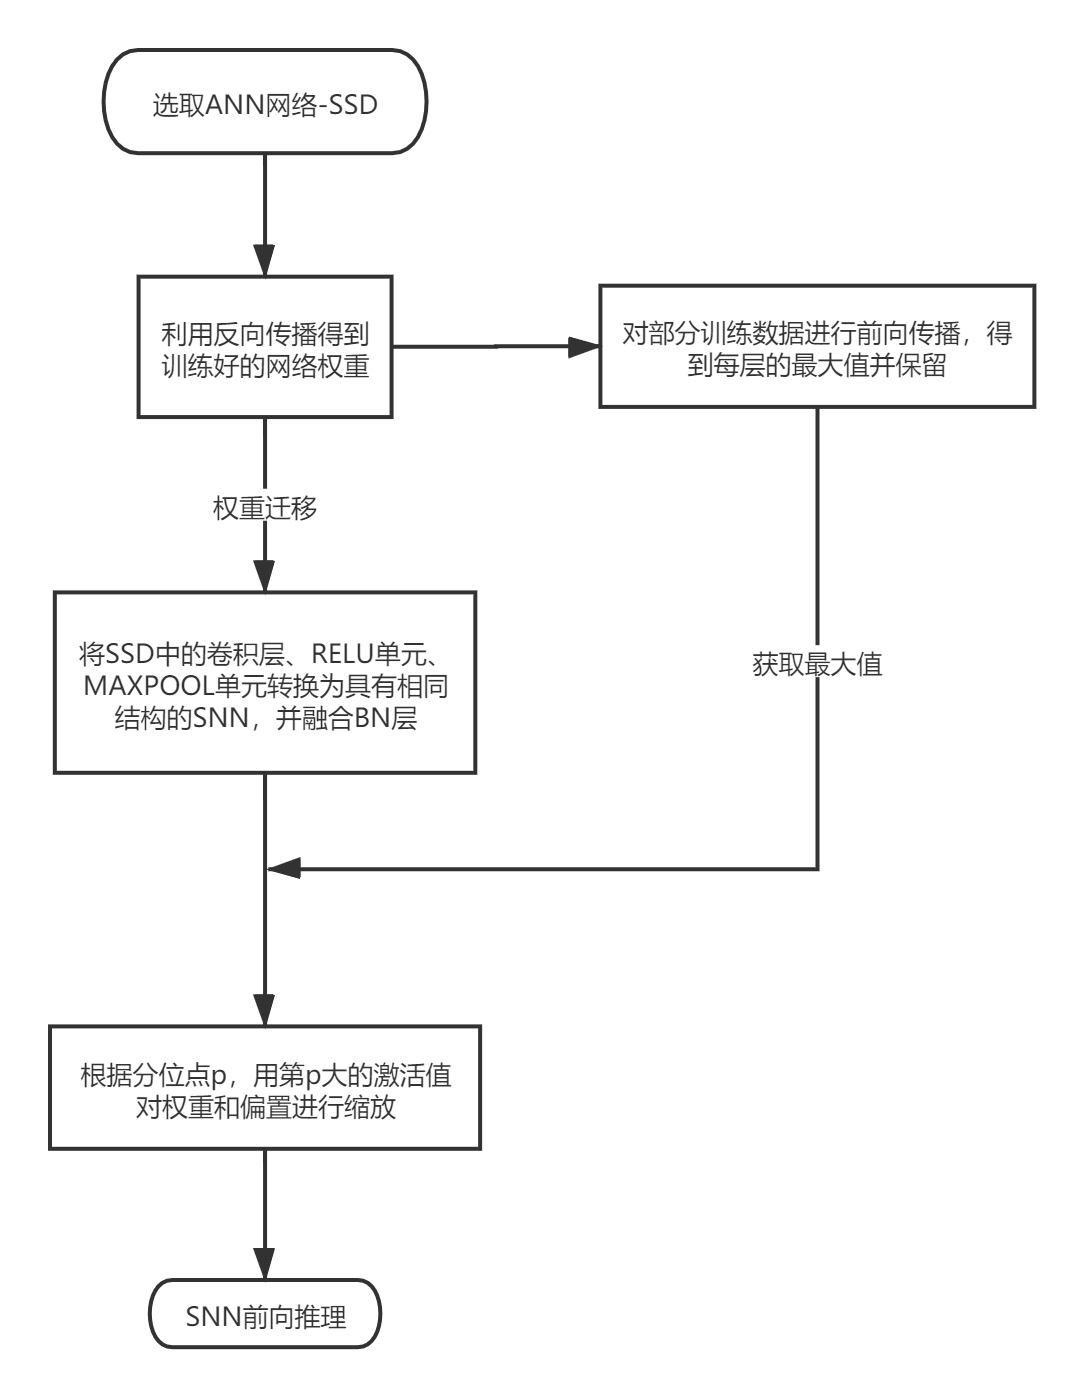
\includegraphics[scale = 0.35]{figures/flowchart.png}
	\caption{实验流程}
\end{figure}
\subsection{获取最大激活值}
\par
根据
\mycitex{2015Fast}提出的$\mathbf{Data-Base\; Normalization}$方法,
由于训练集和测试集服从同一分布,所以从训练集中选出部分图片,用这些图片作为输入,
输入到网络中进行前向传播,获得每一层的最大值,这就是max-norm的方法。实验时,
我们按前文所提到的设置一个百分位数p,
取p值在[99.0,99.999]范围内,选取第p大的激活值,防止个别过大的离群激活值导致发放率过低。
\subsection{等价转换操作}
\par
将原有SSD的四个模块Vgg、Extras、Loc、Conf均等价转换为脉冲单元SpikeUnit,
spikeUnit接收的opration类型有 nn.Conv2d/nn.Linear/nn.BatchNorm2d/nn.MaxPool2d/
nn.AvgPool2d/nn.Dropout/nn.ReLU,conv做运算并且发放脉冲,relu不做运算,而是单纯的积累膜电势并发放脉冲。
Maxpooling取最大的区域内的活动,只允许最大发放率的脉冲通过。
\subsection{前向推理}
\par
当网络转换完毕后,对输入的图片进行处理后,进入网络进行前向传播,即可得到目标置信度和位置的预测值。
这里的神经元采用IF神经元,实值编码,即将脉冲整数转换为浮点数,同时保留膜电势。
多个图片进行推理时,为了前面图片不影响后者图片,对各层中各个神经元进行膜电势、脉冲数、发放脉冲数的重置。
\section{spiking-yolo}
\par
在目标检测任务中,识别多个目标并在它们周围绘制边界框(回归问题)需要高数值精度来预测输出值。当使用常规ANN-SNN转换方法应用于SNN时,其遭受严重的性能降级。
可能的原因有两个:来自分层归一化导致的极低的发放率,以及leaky-RELU功能的中负激活没有办法表示。为此有两种新方法:分别为通道标准化和不平衡阈值的带符号神经元。
\subsection{通道标准化}
\par
为了防止神经元过度激活或过激活,基于数据的标准化技术被提出。逐层归一化\mycitex{2015Fast}(layer-norm)是最着名的技术之一:
基于训练和测试数据集的分布相似的假设,通过运行训练计算出的相应层的最大激活来规范特定层中的权重ANN中的数据集。公式前文中也提及:
\[
\mathbf{W}^l \to \mathbf{W}^l \frac{\lambda^l}{\lambda^{l-1}} and \mathbf{b}^l \to \mathbf{b}^l / \lambda^l
\]
\par
之后\mycitex{2017Conversion}引入了一种方法,该方法通过最大激活的99.9百分位来标准化激活,这为异常值提供了鲁棒性,从而确保了神经元的充分运行。
然而,根据我们的分析,传统的基于数据的归一化方法在应用于对象检测时由于激活不足而遭受显着的性能降级。
因此,我们提出了一种更细粒度的归一化技术,称为信道方向归一化(缩写为信道规范),以便在深度SNN中实现快速有效的信息传输。
我们的方法通过最大可能的激活(第99.9百分位数)以通道方式归一化权重,而不是传统的分层方法,算法如下:

\begin{algorithm}[H]
	\caption{通道标准化}%算法名字
	\SetKwBlock{Begin}{}{end}
	//从训练数据集中的每个通道中,计算最大激活值($\lambda$) \\
	\LinesNumbered %要求显示行号
\For{第 $l$ 层}{
    \For{第 $j$ 输出层}{
		 $\lambda_j^l=max(A_J^l)$ \\
	}
}
	//将通道标准化应用到测试集的推理上 \\
	\For{第 $l$ 层}{
    \For{第 $j$ 输出层}{
		 $\tilde{b}_j^l = b_j^l \; / \; \lambda _j ^l$
		\For{第 $i$ 输入通道}{
			\eIf{$l$ 是第一层}{
				$\tilde{w}_{i,j}^l=w_{i,j}^l \; / \; \lambda_j^l$
			}{
				$\tilde{w}_{i,j}^l=w_{i,j}^l \; / \; \lambda_j^l \; \lambda_i^{l-1}$
			}
		}
	}
}
\end{algorithm}
\par
细化的通道归一化可以提高神经元的发放率,即非常小的激活值被正确归一化,将在更短的时间内准确地传输信息。
实验证明逐通道归一化会使更多的神经元产生大量的脉冲。许多神经元产生高达80%的发放率。这是在逐层归一化上的发放率的很大改进。
这些小的激活可能意义不大,并且在诸如图像分类的简单应用中对网络的最终输出可能具有非常小的影响。但是,小的激活对回归问题至关重要。
\subsection{不平衡阈值的带符号神经元}
\par
ReLU是最常用的激活函数之一,仅保留正输入值,并丢弃所有负值; 
$x>0$时为$f(x)=x$,否则为$f(x) = 0$。与ReLU不同,leaky-ReLU包含具有泄漏项的负值,斜率为α,通常设置为0.01; 
$x>0$时为$f(x)=x$,否则为$f(x) = \alpha x$.
大多数先前的研究都集中在将IF(整合和反射)神经元转换为ReLU功能,并完全忽略了泄漏项。
也就是说,一旦可能包含有用信息的神经元变为负数,那么它将为零,并且所包含的信息在整个网络过程中将是无用的。
但在yolo中,泄露项占了不少的比例,因而不能忽视它,这里提出不平衡阈值的带符号神经元来表示漏项。
\par
可以引入第二个阈值电压$V_{th,neg}$,其等于正阈值电压除以一个负斜率$-\alpha$。公式如下:
\begin{equation}
	fire=(V_{mem}) = \begin{cases}
		1, & \text{if } V_{mem} \ge V_{th,pos}(V_{th}) \\
		-1, & \text{if } V_{mem} \le V_{th,neg}(-\frac{1}{\alpha}V_{th}) \\
		0, & \text{otherwise, no firing}
	\end{cases}
\end{equation}
\par
举个例子,如果$\alpha=0.1$,正激活阈值$V_{th,pos}$为1,则负激活阈值$V_{th,neg}$为-10。也就是负值时的膜电势需要十倍才能超过负阈值,产生脉冲。通过引入额外的阈值电压
来实现泄露项,我们实现了脉冲的离散性,在生物上更合理。
图片展示如下:
\begin{figure}[H]
	\centering
	\setlength{\abovecaptionskip}{0cm}  
	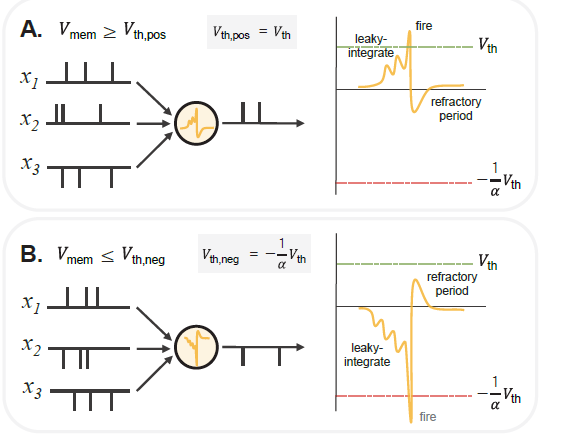
\includegraphics[scale=1]{figures/leakyrelu.png}
	\caption{带符号的不平衡阈值神经元}
\end{figure}
\subsection{解码方式}
\par
前面提到的两种方案,在后续的实验中,如果不应用带符号的不平衡阈值(IBT)神经元,很多的检测结果mAP都极低,
这是因为泄露RELU在tiny-yolo中占比很大。当仅应用具有IBT的带符号的神经元时,它仍然难以检测对象,
大约只有7.3%的mAP\mycite{Spiking-yolo},但这也表明带有IBT的带符号神经元可以补偿泄漏RELU中的泄漏项。
因此,接下来的实验将带有IBT方法的带符号神经元作为默认值来进行。这一部分主要是对解码方式进行讨论。
\par
有两种不同的输出解码方式:一种是基于累积膜电势$V_{mem}$,另一种基于脉冲计数$spike \;count$,脉冲计数$spike \;count$可以简单地由
$V_{mem}$除以$V_{th}$来计算。但是由于$V_{mem}$除以$V_{th}$的商是四舍五入的方式,因此可能出错并且丢失信息。所以基于$V_{mem}$的输出解码
方案在解释脉冲发放时会更加精确,在一些实验中证明\mycite{Spiking-yolo},其在通道和逐层归一化中也会更快地收敛。
